\documentclass[a4paper]{article}
% Preamble
	\usepackage{fullpage} % Package to use full page
	\usepackage{parskip} % Package to tweak paragraph skipping
	\usepackage{tikz} % Package for drawing
	\usepackage{amsmath}
	\usepackage{hyperref}
	\usepackage{amsmath,amssymb}
	\usepackage{color}
	\usepackage[version=4]{mhchem} 
	\usepackage{bm}
	\usepackage{verbatim}
	\usepackage{subfig}
	\usepackage{graphicx}
	\graphicspath{ {./Figures/} }
		
\title{Special Relativity Part 3}
\author{Lauren Shriver}
\date{08/10/2018}

\begin{document}
	\maketitle
	\section*{Overview of Part 2}
		\subsection*{Thought Experiment}
			\subsubsection*{Constants}
				\begin{itemize}
					\item Speed of light: $c \approx 3 \cdot 10^8 \mathrm{m/s}$  
				\end{itemize}
			\subsubsection*{Path Time Diagram and Associated Variables}
				\begin{figure}[!htbp]
					\begin{center}
						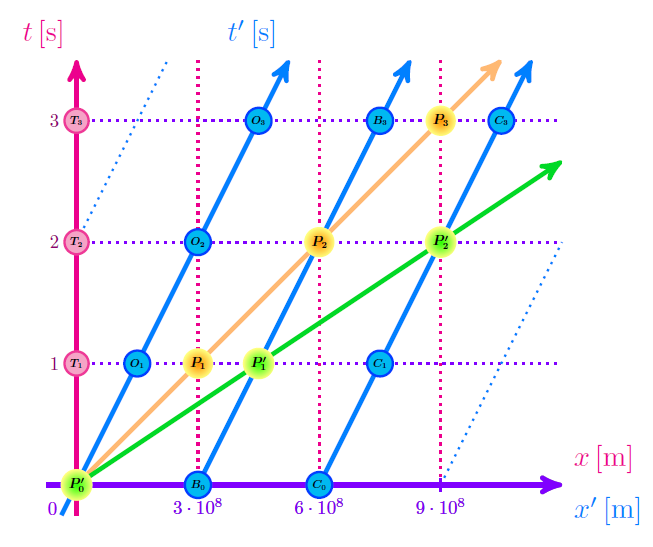
\includegraphics[width=7.5cm]{pathtime1.png}
						\caption{Path-time diagram of the $S'$-frame overlayed on the $S$-frame. $T_i$, $O_i$, $B_i$, and $C_i$ denote Trumps, Obama's, Bush's, and Clinton's position (respectively) at time $t=i$ seconds. $P_i$ denotes the coordinates at time $t=i$ seconds for a photon emitted from Trump's spaceship at time $t=0$ seconds. Similarly, $P'_i$ denotes the coordinates at time $t=i$ seconds for a photon emitted from Obama's spaceship at $t=0$ seconds.}	
						\label{fig:pathtime}
					\end{center}
				\end{figure}
				\begin{itemize}
					\item $S:(x,t)$ frame = inertial frame of reference (FoR) whose $x=0$ coordinate is defined by Trump's position in a space ship traveling at some constant velocity 
					\item $S':(x',t')$ frame = inertial FoR whose $x=0$ coordinate is defined by Obama's position in a separate spaceship traveling at a constant velocity in the positive $x$ direction at a speed $v=0.5c$ relative to Trump's spaceship (i.e., the $S$ frame)
					\item We are also assuming that Bush and Clinton are also on spaceships traveling with the same velocity as Obama
					\begin{itemize}
						\item Specifically, Bush's spaceship is $3\cdot 10^8 \mathbf{m}$ in front of Obama's spaceship and Clinton's spaceship is $3\cdot 10^8 \mathbf{m}$ in front of Bush's spaceship (with respect to the $x$ axis) 
					\end{itemize}
				\end{itemize}						
		\subsubsection*{Conundrum}
		According to Newtonian/classical/Galilean physics, if Trump and Obama were to simultaneously measure the speed of either photon 1 or photon 2, they should obtain different results. Specifically, since the speed of Obama's spaceship is greater than Trump's, Trumps should measure the speed of either photon as being faster than Obama's measurements would indicate.
		\begin{itemize}
			\item Trump (or, an observer in the $S$ frame) should measure the speed of photon 1 as being $3 \cdot 10^8 \, \mathrm{m/s}$ and the speed of photon 2 as being $6 \cdot 10^8 \, \mathrm{m/s}$
			\item Obama (or, an observer in the $S'$ frame) should measure the speed of photon 1 as being $1.5 \cdot 10^8 \, \mathrm{m/s}$ and the speed of photon 2 as being $3 \cdot 10^8 \, \mathrm{m/s}$
			\item Trump
		\end{itemize}
		As it turns out, in reality both Trump and Obama will measure both photons as traveling with a speed of approximately $3 \cdot 10^{8} \, \mathrm{m/s}$. But this directly contradicts Newtonian mechanics! 
		\begin{itemize}
			\item This has something to do with light always traveling at $3 \cdot 10^8 \, \mathrm{m/s}$ in a vacuum (however, it isn't slowed down by much in a non-vacuum)
		\end{itemize}
	\subsection*{Review of Newtonian Physics}
		\subsubsection*{Assumptions}
		\begin{itemize}
			\item Time is absolute (i.e., one second for Trump is equivalent to one second for Obama - if they both had "perfectly" working watches, they remain synchronized)
			\item Space is absolute (i.e., one meter on Trump's spaceship is equivalent to one meter on Obama's spaceship)
			\item Space and time are two different phenomena 
			\begin{itemize}
				\item Should be able to "travel" in the time direction without moving in the space direction and vice-versa
				\item Thus, space and time are independent, regardless of what FoR you're in
			\end{itemize}
		\end{itemize}
	As it turns out, all these assumptions start to break down at high speeds (maybe also at lower speeds, we just don't/can't detect them). As we begin to consider concepts from relativity, we begin to see that neither space nor time is absolute.  Moreover, we should start to think of any event as occurring in a continuum called \textbf{spacetime}. 
\section*{Minkowski Spacetime Diagrams}
	\subsection*{Readjusting the Path-Time Diagram}
	If space and time are the same thing, why are we using different units (meters for space and seconds for time)?
		\begin{itemize}
			\item Let's scale the time axis by the speed of light to convert one unit. This will convert one unit length along the $t$ axis from $1 \, \mathrm{s}$ to $3 \cdot 10^2 \, \mathrm{m}$.
		\end{itemize}
\end{document}

